% Intended LaTeX compiler: pdflatex
\documentclass[preprint,12pt]{elsarticle}
\usepackage{graphicx}
\usepackage{rotating}
\journal{Computer Physics Communications}
\usepackage[utf8]{inputenc}
\usepackage[T1]{fontenc}
\usepackage{lmodern}
\usepackage{microtype}
\usepackage{amssymb,amsmath}
\usepackage{booktabs}
\usepackage{tabularx}
\usepackage{array}
\usepackage{xurl}
\usepackage{listings}
\usepackage{hyperref}
% elsarticle 3.3 expands affiliation fields and breaks the accent in authors.tex.
\ExplSyntaxOn
\DeclareDocumentCommand \ca_aff_city { O{,} m }
  {
    \csgappto { ca_affiliation_values } { \unexpanded{#2} #1\ca_affitem_postskip }
  }
\ExplSyntaxOff

\lstset{
  basicstyle=\ttfamily\footnotesize,
  breaklines=true,
  columns=fullflexible,
  keepspaces=true,
  showstringspaces=false,
  frame=none,
  aboveskip=0.6em,
  belowskip=0.4em
}
\date{\today}
\title{CON 3.1: a versioned text checkpoint for saddle searches and long-timescale simulations, with its reference implementation readcon-core}
\hypersetup{
 pdfauthor={Rohit Goswami},
 pdftitle={CON 3.1: a versioned text checkpoint for saddle searches and long-timescale simulations, with its reference implementation readcon-core},
 pdfkeywords={checkpoint, specification, interoperability, reproducibility, saddle, restart, eOn},
 pdflang={English}}
\begin{document}

\begin{frontmatter}

%% elsarticle author block. One affiliation.
\author[tt]{Rohit Goswami\fnref{orcid}}
\ead{rgoswami@ieee.org}
\fntext[orcid]{ORCID: 0000-0002-2393-8056.}
\affiliation[tt]{organization={TurtleTech ehf.},
            city={Reykjav\'ik},
            country={Iceland}}


\begin{abstract}
Rare-event campaigns stop and restart through a text checkpoint, and a reader can silently drop a per-axis constraint, an atom identity, or the time unit of a velocity.
CON is the frame eOn uses for minima, saddles, band images and restarts, and the frame ASE reads and writes, yet it grew up inside eOn and was never specified, so those readers diverged.
CON 3.1 is a versioned specification of that frame, with compatibility rules, a grammar and a schema, and readcon-core 0.17.0 is its reference implementation.
eOn 3.6.0 reads CON through this library and has no other CON parser.
A checkpoint written by the default printer reads back bit-identical.
An interrupted eOn band resumed from that checkpoint agrees with the uninterrupted band to \(1\times10^{-14}\,\text{\AA}\), whereas the same frame printed at six decimals drifts by \(5\times10^{-7}\,\text{\AA}\).
Velocities kept in the natural unit and misread as femtoseconds scale the kinetic energy by 103.64.
The Rust core reads at 1.09\,GB/s.
The specification, the implementation and the conformance corpus are released under the MIT licence.

\noindent
\textit{Program title:} readcon-core\\
\textit{CPC Library link to program files:} (to be added by Technical Editor)\\
\textit{Developer's repository link:} \url{https://github.com/lode-org/readcon-core}\\
\textit{Licensing provisions:} MIT\\
\textit{Programming language:} Rust, C, C++, Python, Julia, Fortran 2008\\
\textit{Supplementary material:} normative specification, PEG grammar, JSON schema, conformance corpus, evidence scripts\\
\textit{Nature of problem:}
Campaigns exchange geometries and resume from CON frames, which had no specification.
Readers therefore drop a per-axis mask, drop the atom id after the file has grouped atoms by element, mislabel the velocity time unit, or round coordinates to a fixed number of decimals.
The search that continues then runs under a different constraint, pairs a different atom with its image, or restarts from a different kinetic energy than the one that was stored.
The missing object is a specification of the frame those programs already pass around.
\textit{Solution method:}
CON 3.1 names a major version and a minor version, and it states which later changes a reader of the same major must still accept.
Decimal fields are read with correct rounding, and the default writer emits the shortest text that parses back to the same binary64 value.
Six fixed decimals remain available only when a caller asks for them.
One C ABI sits over the Rust core, so that every binding shares a single parse, and eOn already reads through that path.
A multi-frame file is split by a serial scan of frame boundaries, after which each frame is parsed as its own task and returned in file order.
gzip and zstd are envelopes around the same text.
Unknown metadata keys are kept on rewrite, and an unknown section belonging to a newer minor can be skipped when its width is declared.
\textit{Additional comments including restrictions and unusual features:}
Optional remote-procedure, metatensor and DLPack features are outside this release.
Automatic threading is present when the library is built with the parallel feature, which is how the wheels and the C archives are built.
The Python binding constructs one object per atom while it holds the interpreter lock, after the parse itself has released that lock.
A failed C read returns a null handle and does not classify the error.
% CHECK: update if per-class C error codes ship on the read path.
\end{abstract}

\begin{keyword}
checkpoint \sep specification \sep interoperability \sep reproducibility \sep saddle \sep restart \sep eOn
\end{keyword}

\end{frontmatter}

\section{Introduction}
\label{sec:introduction}
Rare events in solids and molecules set the rates of diffusion, reaction and structural change, and harmonic transition-state theory estimates such a rate from the barrier and from the curvatures at a minimum and at a first-order saddle \cite{eyringActivatedComplexChemical1935,vineyardFrequencyFactorsIsotope1957,hanggiReactionrateTheoryFifty1990}.
The stationary points are found by double-ended searches, among them the nudged elastic band and its climbing-image form, and by single-ended searches such as the dimer, which have been compared as one family of saddle methods on a landscape of minima \cite{henkelmanMethodsFindingSaddle2000,jonssonNudgedElasticBand1998,henkelmanClimbingImageNudged2000,henkelmanDimerMethodFinding1999,olsenComparisonMethodsFinding2004,walesExploringEnergyLandscapes2018}.
When the event is too rare for a direct trajectory, the same physics is reached by hyperdynamics and other accelerated molecular dynamics, by adaptive kinetic Monte Carlo, and by farming parallel replicas \cite{voterHyperdynamicsAcceleratedMolecular1997,voterExtendingTimeScale2002,mironAcceleratedMolecularDynamics2003,henkelmanLongTimeScale2001,voterIntroductionKineticMonte2007,novotnyMonteCarloAlgorithms1995,voterParallelReplicaMethod1998,perezLongtimeDynamicsThrough2016}.
Basin hopping and minima hopping propose the next minimum on that landscape, so a campaign is a sequence of searches that must be able to stop \cite{walesGlobalOptimizationBasinhopping1997,goedeckerMinimaHoppingEfficient2004}.
Stopping is part of the calculation, not an interruption of it.
A rate that takes a laboratory time to observe is assembled from many short runs, and each run has to begin from a geometry the previous run actually stored.
The file is therefore not a log of the search but the state the next search is allowed to trust.

Each of those searches calls a force evaluator many times, and the geometry between calls is a file rather than a region of shared memory.
A queue preempts the job, a stateless server hands the geometry to a client as text, a public-resource client returns a finished task, and a distributed adaptive kinetic Monte Carlo rank farms the next escape \cite{andersonBoincSystemPublicresource2004,pedersenDistributedImplementationAdaptive2010}.
eOn \cite{goswamiEonV3602026}, described in the older eOn paper \cite{chillEonSoftwareLong2014} and in a thesis chapter on the rewrite \cite{goswamiEfficientExplorationChemical2025}, is the code in which this text became the working checkpoint.
A surrogate fitted to earlier force calls can propose the next saddle step inside that loop, so the geometry still has to land on a force evaluator that reads the frame \cite{goswamiEfficientImplementationGaussian2025,koistinenNudgedElasticBand2019}.
In practice the checkpoint is shared state: another rank, another machine, or a Python hand-off may be the next reader, and a result that cannot be restarted from a defined file is not one another group can rerun \cite{pengReproducibleResearchComputational2011,inceCaseOpenComputer2012}.
Caring for that file means it still means the same thing after the code that wrote it has changed, which is the point at which an unspecified format collapses into whatever the last reader happened to implement \cite{hinsenCaringYourData2012,hinsenDealingSoftwareCollapse2019}.
We therefore treat the checkpoint as part of the method.
A distributed client never shares the writer's memory, so the bytes on disk are the only state the next force call will see, whether the wait was a queue, a copied file on another machine, or a hand-off into Python.
Long-timescale work makes the same demand, because an accelerated trajectory or a kinetic Monte Carlo campaign stops many times before a laboratory rate is visible, and each of those stops is a read of this file rather than a resume of a living process.

CON carries minima, saddles, images of a band and the restart of a search.
The Atomic Simulation Environment, which began as a scripting interface to an electronic-structure code, reads and writes the same text \cite{bahnObjectorientedScriptingInterface2002}.
The older eOn paper describes the code, not the file, and the file was never specified, so the eOn reader and the ASE reader diverged \cite{goswamiEonV3602026,chillEonSoftwareLong2014}.
Six fixed decimals move a coordinate by up to \(5.0\times10^{-7}\,\text{\AA}\) on a write, while a shortest round-trip printer returns the same binary64 value.
Velocities in eOn and in ASE are stored in the natural unit \((\mathrm{amu}\cdot\text{\AA}^{2}/\mathrm{eV})^{0.5}=10.1805\,\mathrm{fs}\), and producers of the 3.0 era labelled that unit fs, so a trusting reader scales the kinetic energy by 103.64.
ASE turns any nonzero fourth-column mask into a full freeze and ignores the fifth-column identity, so a height constraint becomes a frozen atom and atoms that the file grouped by element are paired by row.

H5MD, extended XYZ and the ASE trajectory store already keep positions, and in places an identity, a constraint object or a grammar \cite{buylH5mdStructuredEfficient2014}.
None of them is the readable frame this campaign already exchanges, so Section~\ref{sec:format} sets that combination beside those formats rather than treating the names as substitutes.
Chemical markup, the Protein Data Bank, package-independent parsers and molecular viewers established the habit of a documented exchange, while a live coupling such as i-PI or the MolSSI driver interface moves coordinates without leaving a file that a stopped job can resume from \cite{murrayrustChemicalMarkupXml1999,bermanProteinDataBank2000,bermanAnnouncingWorldwideProtein2003,oboyleCclibLibraryPackageindependent2008,verstraelenIodataPythonLibrary2021,humphreyVmdVisualMolecular1996,ceriottiIpiPythonInterface2014,litmanIpi30Flexible2024,barnesMolssiDriverInterface2021}.

We present four contributions.
(i) CON 3.1 is a versioned specification with compatibility rules, a parsing-expression grammar and a JSON schema.
(ii) readcon-core 0.17.0 is a reference implementation with one C ABI and five bindings, and eOn 3.6.0 reads CON through it \cite{goswamiEonV3602026}.
(iii) One conformance corpus is run by every binding, so a legal frame and an illegal frame are decided in common.
(iv) We compare an interrupted eOn band, resumed from both printers, with the uninterrupted run \cite{goswamiEonV3602026,goswamiEnhancedClimbingImage2026}, and we place the cost of the read next to a force call.
Six requirements follow, and Section~\ref{sec:requirements} ties each one to a failure: a per-axis constraint (R1), a persistent atom identity (R2), a declared velocity time unit (R3), an exact floating-point round trip unless the caller asks for fixed decimals (R4), metadata a later minor can extend (R5), and text a person can inspect after a job has stopped (R6).
Section~\ref{sec:format} specifies the frame, Section~\ref{sec:implementation} describes the library, Section~\ref{sec:validation} reports the corpus and the eOn restarts, and Section~\ref{sec:performance} reports that cost.
Figure~\ref{fig:workflow} is the path.

\begin{figure}[ht]
\centering
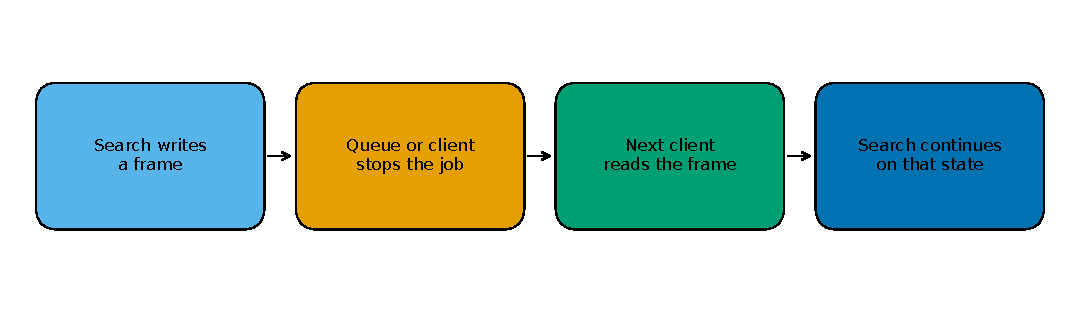
\includegraphics[width=\textwidth]{figures/generated/workflow.pdf}
\caption{A rare-event campaign treats the checkpoint as shared state.
The search writes a frame, the job stops on a queue or a remote client, and the next reader loads that frame before the following force calls.
What the frame dropped is what the resumed search silently gets wrong.}
\label{fig:workflow}
\end{figure}

\section{What a rare-event checkpoint must carry}
\label{sec:requirements}
A restarted rate is only as faithful as the free modes, the atom pairing and the kinetic energy the frame still carries.
Table~\ref{tab:requirements} puts the six requirements against the failure each one closes.

\begin{table}[ht]
\centering
\small
\caption{Requirements on a rare-event checkpoint, the failure each one closes, and the quantity that then changes.}
\label{tab:requirements}
\begin{tabular}{p{0.22\linewidth}p{0.36\linewidth}p{0.32\linewidth}}
\toprule
Requirement & Failure & What changes \\
\midrule
R1 per-axis mask & Nonzero column 4 becomes a full freeze & Free modes of the prefactor, and whether a hop exists \\
R2 persistent id & Type grouping pairs atoms by row & Which atom is aligned with its image \\
R3 declared time unit & Natural-unit velocities labelled fs & Kinetic energy on restart, by \(103.64\) \\
R4 float round trip & Six fixed decimals & Coordinates, by up to \(5.0\times10^{-7}\,\text{\AA}\) \\
R5 extendable metadata & Unknown keys dropped on rewrite & Bead index, energy, potential name \\
R6 inspectable text & A binary container needs a decoder & Whether a dead job can be diagnosed \\
\bottomrule
\end{tabular}
\end{table}

Coordinates printed to six digits after the decimal move by as much as half a unit in the seventh digit, which is \(5.0\times10^{-7}\,\text{\AA}\) on the checkpoint measured in Section~\ref{sec:validation}.
A later force call then sees a different geometry, and a chain of such writes walks the atoms even when the optimiser itself has not stepped.
The default printer avoids that walk by emitting text that parses back to the same binary64 value, so the only geometry change on a restart is the one the search intends.
On the nine-atom frame of Listing~\ref{lst:frame} the six-decimal form is the readable one, and Section~\ref{sec:format} records what that readability costs in energy as well as in position.

Velocities are the second silent change, because kinetic energy scales with the square of the unit in which they are stored.
Here \(1\,\text{\AA}=10^{-10}\,\mathrm{m}\), \(1\,\mathrm{fs}=10^{-15}\,\mathrm{s}\) and \(1\,\mathrm{eV}=1.602176634\times10^{-19}\,\mathrm{J}\).
The natural unit shared by eOn and ASE is \((\mathrm{amu}\cdot\text{\AA}^{2}/\mathrm{eV})^{0.5}\), equal to \(10.1805\,\mathrm{fs}\) once the constants that define the electronvolt and the atomic mass unit are inserted \cite{tiesingaCodataRecommendedValues2021,mckeeverUnitMeasurementLibraries2021}.
Producers of the 3.0 era wrote the natural-unit numbers and labelled the unit fs, so a reader that honours the label divides every component by \(10.1805\) and multiplies the kinetic energy by \(103.64\).
A velocity Verlet step and a velocity-rescaling thermostat both advance those components, therefore the label has to travel with them or the restarted temperature is a different temperature \cite{swopeComputerSimulationMethod1982,bussiCanonicalSamplingThrough2007}.
Section~\ref{sec:validation} shows the factor on a 28-atom slab at 300\,K, and it is an illustration of the mislabel rather than a dynamics validation, because an eOn dynamics job redraws velocities and writes none.

A surface calculation freezes buried atoms on every axis and often holds only the height of an adsorbate, which is a different constraint from a full freeze \cite{jonssonSimulationSurfaceProcesses2011,larsenAtomicSimulationEnvironmenta2017}.
Harmonic transition-state theory builds the prefactor from the free modes at the minimum and at the saddle, so an axis that was meant to move and is instead frozen removes a mode, and an axis that was meant to be held and is instead free adds one.
On the slab of Section~\ref{sec:validation} the bottom nine atoms carry mask 7 and the adatom carries mask 4, meaning \(z\) only.
ASE 3.29.0 reads every nonzero mask as a full freeze, which pins the adatom on \(x\) and \(y\) as well, so the band cannot represent a hollow-to-hollow hop and the free-mode count of the prefactor changes with it.
% CITE-NEEDED: ASE 3.29.0 as a software release has no DOI in the citation list.
The same optimiser state is a separate loss: limited-memory quasi-Newton, the optimisers surveyed for saddle searches, and damped molecular dynamics such as FIRE all keep a short history that a geometry frame does not store \cite{nocedalUpdatingQuasinewtonMatrices1980,sheppardOptimizationMethodsFinding2008,bitzekStructuralRelaxationMade2006}.
A resume can therefore match the coordinates and still take a different next step, which is the L-BFGS control in Section~\ref{sec:validation}.

Identity is the remaining pairing, and images of a band are compared atom by atom.
A shape-matching method such as iterative rotational alignment needs a stable correspondence once the file has grouped atoms by chemical symbol \cite{gundeIraShapeMatching2021}.
Column 5 is that correspondence, kept on the row so a later frame can find the same atom after the grouping.
Without it, two frames that list carbon before nitrogen before hydrogen will pair whatever sits on the same row, even when the hydrogen in one frame is not the hydrogen in the next.
A parallel-replica segment has the same need, since a dephased copy is the same atoms and not a new indexing \cite{perezParallelReplicaDynamics2015}.
R5 and R6 are what let a campaign attach a bead index or an energy without waiting for every reader, and what let a person see a mask after the job has died, which is why the specification below stays text.

\section{The CON 3.1 format}
\label{sec:format}
A CON file is a sequence of text frames.
Listing~\ref{lst:frame} is nine platinum atoms in a \(2\times2\times2\) cell with one adatom, and the velocities sit in the natural unit because that is what line 2 declares.

\begin{lstlisting}[caption={A nine-atom Pt frame in CON 3.1. Line 2 declares the natural time unit for the velocity block. Velocity rows for ids 1 to 7 are omitted, as the note in the listing says.},label={lst:frame}]
Pt(100) 2x2x2 with one Pt adatom
{"con_spec_minor":1,"con_spec_version":3,"pbc":[true,true,false],"sections":["velocities"],"units":{"energy":"eV","length":"angstrom","mass":"amu","time":"(amu*angstrom^2/eV)^0.5"}}
5.5437171645025325e0 5.5437171645025325e0 1.396e1
9e1 9e1 9e1


1
9
1.95084e2
Pt
Coordinates of Component 1
1.3859292911256331e0 1.3859292911256331e0 6e0 7 0
4.1577878733769e0 1.3859292911256331e0 6e0 7 1
1.3859292911256331e0 4.1577878733769e0 6e0 7 2
4.1577878733769e0 4.1577878733769e0 6e0 7 3
0e0 0e0 7.96e0 0 4
2.7718585822512662e0 0e0 7.96e0 0 5
0e0 2.7718585822512662e0 7.96e0 0 6
2.7718585822512662e0 2.7718585822512662e0 7.96e0 0 7
1.3859292911256331e0 1.3859292911256331e0 9.76e0 4 8

Pt
Velocities of Component 1
1.4685859972256804e-3 6.275175116609037e-4 -1.8115929554652053e-3 7 0
... (rows for ids 1-7 are omitted in the paper with a note) ...
3.748769356553213e-3 2.43327727576049e-3 -1.3238979663774354e-3 4 8
\end{lstlisting}

Line 1 is free text naming the frame.
Line 2 is a single JSON object, without a byte-order mark, holding the version, the units, the periodicity and the names of the sections that follow \cite{brayJavascriptObjectNotation2017}.
Lines 3 and 4 are the three cell lengths and the three angles in degrees.
Two blank lines are the free-text pair a version 1 file also carries, after which the type count, the per-type counts and the masses appear: one type, nine atoms, mass \(195.084\,\mathrm{u}\).
Coordinates then come as a symbol, the heading ``Coordinates of Component \(N\)'', and one row of \(x\), \(y\), \(z\), mask and id per atom.
A single blank line opens the velocity block, which repeats the symbol under ``Velocities of Component \(N\)'' and copies the mask and the id onto each row.
A value near \(1.386\) is printed as \texttt{1.3859292911256331e0}, and that \texttt{e0} form is genuinely harder to scan than a fixed decimal.
Six decimals turn the first row into \texttt{1.385929 1.385929 6.000000 7 0}, which a person can check by eye and which no longer parses back to the stored bits.
Under version 1, line 2 is a comment, column 4 is only 0 or 1, and masks 7 and 4 cannot be stored as written.

\subsection{Cell}
Lengths and angles rebuild the box once the vectors are placed, with \(a\) along \(x\) and \(b\) in the \(xy\) plane,
\begin{equation}
\mathbf{a}=a\,\hat{\mathbf{x}},\qquad
\mathbf{b}=b\cos\gamma\,\hat{\mathbf{x}}+b\sin\gamma\,\hat{\mathbf{y}},
\end{equation}
after which \(\mathbf{c}\) is fixed by \(\alpha\) and \(\beta\) so the cell is right-handed \cite{bekkerUnificationBoxShapes1997}.
When line 2 also carries \texttt{lattice\_vectors}, those three rows are the cell and they win on read, while lines 3 and 4 are kept consistent with them.
A missing periodicity flag means the cell is periodic along every axis.

\subsection{Mask and identity}
From version 2, column 4 is the three-bit integer in Table~\ref{tab:mask}: bit 0 is \(x\), bit 1 is \(y\) and bit 2 is \(z\).
Mask 0 is free, mask 4 holds \(z\) only, and mask 7 holds every axis.
Version 1 stores 0 or 1 in that column, and 1 means fully fixed, so a version 1 writer cannot represent the adatom without freezing it on \(x\) and \(y\) as well.
A float spelling, a sign, or a value outside the legal set is an illegal flag in every mode, including when strict validation is off.

\begin{table}[ht]
\centering
\small
\caption{Mask bits from version 2. Version 1 stores 0 (free) or 1 (fixed on \(x\), \(y\) and \(z\)) in the same column.}
\label{tab:mask}
\begin{tabular}{ccc}
\toprule
Bit & Axis & Value \\
\midrule
0 & \(x\) & 1 \\
1 & \(y\) & 2 \\
2 & \(z\) & 4 \\
\bottomrule
\end{tabular}
\end{table}

Column 5 is an integer from 0 through \(2^{64}-1\), read as an integer rather than through binary64, and writers emit ids unique in the frame.
Repeated ids keep file order, and unique ids sort, ascending, into the order from before the file grouped atoms by element.
A four-column row takes its id from the zero-based row index.
This release returns file order from the core and the bindings, while the core can still compute the pre-grouping permutation.
% CHECK: update if the bindings return pre-grouping order rather than file order.

\subsection{Metadata, versions and errors}
Table~\ref{tab:keys} is the 25 reserved keys, and unknown keys survive a rewrite.
An unknown minor of a known major is accepted and an unknown major is rejected, including JSON majors 0 and 1.
An unknown section on a newer minor may be skipped when \texttt{section\_arity} gives its width.
Setting \texttt{validate} true checks key types, a positive cell and a section list, and it does not relax checks that already apply.

\begin{table}[ht]
\centering
\footnotesize
\caption{Reserved metadata keys on line 2 and their JSON types.}
\label{tab:keys}
\begin{tabular}{ll@{\hspace{1.5em}}ll}
\toprule
Key & Type & Key & Type \\
\midrule
\texttt{con\_spec\_version} & int & \texttt{neb\_bead} & int \\
\texttt{con\_spec\_minor} & int & \texttt{neb\_band} & int \\
\texttt{section\_arity} & object & \texttt{convergence\_fmax} & number \\
\texttt{sections} & array & \texttt{convergence\_energy} & number \\
\texttt{validate} & bool & \texttt{converged} & bool \\
\texttt{generator} & string & \texttt{fmax} & number \\
\texttt{units} & object & \texttt{bonds} & array \\
\texttt{pbc} & array & \texttt{storage\_dtypes} & object \\
\texttt{lattice\_vectors} & array & \texttt{chemfiles\_atom\_names} & array \\
\texttt{energy} & number & \texttt{chemfiles\_atom\_types} & array \\
\texttt{potential} & object & \texttt{chemfiles\_atom\_properties} & array or object \\
\texttt{frame\_index} & int & & \\
\texttt{time} & number & & \\
\texttt{timestep} & number & & \\
\bottomrule
\end{tabular}
\end{table}

From minor 1, dated 11 October 2026 in Table~\ref{tab:versions}, a velocities block must declare \texttt{units.time}, spelled \texttt{(amu*angstrom\^{}2/eV)\^{}0.5} for the natural unit.
Versions 1, 2 and 3.0 are read as the natural unit, and an fs label on those files is not trusted.
Accepting an unknown minor and rejecting an unknown major is the split H5MD uses for its own major and minor \cite{buylH5mdStructuredEfficient2014}.

\begin{table}[ht]
\centering
\small
\caption{CON versions. Dates are the days the corresponding rules were fixed.}
\label{tab:versions}
\begin{tabular}{p{0.12\linewidth}p{0.22\linewidth}p{0.58\linewidth}}
\toprule
Version & Date & Change \\
\midrule
1 & original eOn text & Column 5 present; column 4 is 0 or 1; no JSON. \\
2 & 2026-03-25 & JSON line 2, ids, bit masks, declared sections. \\
3.0 & 2026-06-27 & \texttt{units.length} and \texttt{units.energy} required; no minor. \\
3.1 & 2026-10-11 & Minor 1; \texttt{units.time} required with velocities; natural-unit rule for older files. \\
\bottomrule
\end{tabular}
\end{table}

Each failure belongs to a class: missing version, malformed metadata, a non-finite number, an illegal flag, a bad count, an illegal unit, a short header, a short coordinate block, a short or missing section, a bad number, a row of the wrong width, an unknown section, an unsupported version, or a failed strict check.
Several failures resolve to the lowest line, counting metadata as line 2, so a parallel read names the same failure.

\subsection{Sections}
A section exists when \texttt{sections} names it.
With no such key, one blank line that begins a complete velocity block is still a velocity section, and exactly one blank line precedes every later section.
Table~\ref{tab:sections} is the set reserved at minor 1: three values for a vector, one for a scalar, then the flag and the id.
Displacements and spreads use \texttt{units.length}, every spread component is at least zero, and the per-atom energies are named \texttt{energies}.
A metadata energy need not match their sum.
A new reserved name raises the minor, not the major.

\begin{table}[ht]
\centering
\small
\caption{Reserved sections at minor 1. Each data row is the value fields, then the flag and the id.}
\label{tab:sections}
\begin{tabular}{lll}
\toprule
Section & Values & Notes \\
\midrule
Velocities & \(v_x\, v_y\, v_z\) & Time unit from minor 1 \\
Forces & \(f_x\, f_y\, f_z\) & \\
Energies & one value & Section name \texttt{energies} \\
Charges & one value & \\
Spins & one value & \\
Magmoms & \(m_x\, m_y\, m_z\) & \\
Displacements & \(d_x\, d_y\, d_z\) & \texttt{units.length} \\
Spreads & \(s_x\, s_y\, s_z\) & \texttt{units.length}, each \(\geq 0\) \\
\bottomrule
\end{tabular}
\end{table}

\subsection{Floating-point text}
Readers convert each finite decimal to binary64 with correct rounding \cite{ieeecomputersocietyIeeeStandardFloatingpoint2019,goldbergWhatEveryComputer1991,clingerHowReadFloating1990,clingerHowReadFloating2004}.
The default writer prints a shortest decimal that parses back to the same value, in the line of shortest printers that runs from the early algorithms through Grisu, Errol and Ry{\=u} \cite{steeleHowPrintFloatingpoint1990,steeleHowPrintFloatingpoint2004,burgerPrintingFloatingpointNumbers1996,loitschPrintingFloatingpointNumbers2010,andryscoPrintingFloatingpointNumbers2016,adamsRyFastFloattostring2018}.
On the eOn checkpoint of Section~\ref{sec:validation} that text reads back bit-identical, whereas six decimals move a coordinate by up to \(5.0\times10^{-7}\,\text{\AA}\), and on Listing~\ref{lst:frame} they shift positions by at most \(4.2\times10^{-7}\,\text{\AA}\) and an EMT energy by \(4.4\times10^{-7}\,\mathrm{eV}\).

\subsection{Compression and older producers}
gzip and zstd wrap the same bytes, they are recognised by magic rather than only by a file name, and every gzip member is read in order \cite{deutschGzipFileFormat1996,colletZstandardCompressionApplicationzstd2021}.
Version 1 and version 2 producers, including the eOn velocity writer, still emit six fixed decimals.
That lossy form is opt-in in this release (\texttt{precision=6}), because the default writer is the round-trip printer.
The reading claim stops there: eOn 3.6.0 reads CON through this library, and its velocity writer is still the six-decimal one.

\subsection{Related formats}
H5MD stores a trajectory in HDF5 with a major, a minor, an id element, and facilities for compression and slicing \cite{buylH5mdStructuredEfficient2014,folkOverviewHdf5Technology2011}.
TNG, TRR, XTC, DCD, AMBER NetCDF (angstrom, picosecond, convention version 1.0) and ADIOS record a finished run, so their time is a dataset or a convention rather than a mask on the text a saddle search reloads \cite{lundborgEfficientExtensibleFormat2014,spangbergTrajectoryNgPortable2011,rewNetcdfInterfaceScientific1990,brownSoftwarePortableScientific1993,godoyAdios2Adaptable2020,weikEspresso40Extensible2019}.
% CITE-NEEDED: the AMBER NetCDF convention has no DOI in the citation list.

POSCAR selective dynamics is per-axis, while atom order follows the species counts, so a surviving id is not part of that geometry \cite{kresseEfficientIterativeSchemes1996}.
Extended XYZ has a grammar, an ASE trajectory stores \texttt{FixCartesian} objects, and CIF, mmCIF, PDB and a LAMMPS dump name an archive atom or leave the unit style outside the snapshot \cite{thompsonLammpsFlexibleSimulation2022}.
% CITE-NEEDED: the extended XYZ specification has no DOI in the citation list.

Converters and multi-format readers keep a column only when the dialect defined it, so the mask's meaning often lives in the tool \cite{hirelAtomskToolManipulating2015,oboyleOpenBabelOpen2011,meyerEssentialDynamicsTool2006,stukowskiVisualizationAnalysisAtomistic2010}.
The specification puts that rule in the frame, so a new binding does not invent a second reading of column 4.
i-PI and the MolSSI driver interface pass coordinates to a force engine and leave no file, so a stopped job has nothing to resume from \cite{ceriottiIpiPythonInterface2014,litmanIpi30Flexible2024,barnesMolssiDriverInterface2021}.
Live coupling moves a running step, and it does not replace the checkpoint a queue will reload.
TREXIO stores a wave function in text or in HDF5, a different record from this geometry checkpoint \cite{posenitskiyTrexioFileFormat2023,smithMolssiQcarchiveProject2021,hinsenMosaicDataModel2014}.
A repository keeps the finished saddle for publication, after the restart file has already done its job.

Table~\ref{tab:formats} sets eight formats against ten features.
CON 3.1 is the only row joining a per-axis mask, a persistent id, a declared time unit, a float round-trip rule and a grammar plus schema in one readable frame, and the claim is that combination.
H5MD's version pair and id element, AMBER NetCDF's unit convention, POSCAR selective dynamics, the extended XYZ grammar, ASE constraint objects and TREXIO's two back ends are each older than the row.

\begin{sidewaystable}
\centering
\scriptsize
\caption{Eight formats against ten restart features, each cell taken from the public specification of that format.
``Partial'' means the neighbouring field exists under a narrower rule.
``Objects'' means the constraint is stored as a serialised constraint object.}
\label{tab:formats}
\begin{tabular}{p{2.5cm}*{8}{p{1.55cm}}}
\toprule
 & CON 3.1 & Legacy CON & extxyz & ASE .traj & H5MD & AMBER NetCDF & LAMMPS dump & POSCAR \\
\midrule
Text or binary & text & text & text & binary & binary & binary & text & text \\
Versioned spec & yes & no & no & yes & major/minor & version 1.0 & no & no \\
Id survives reorder & yes & column 5 & no & not stated & id element & no & if requested & no \\
Per-axis constraint & yes & 0 or 1 & not stated & yes, as objects & no & not stated & no & selective dynamics \\
Velocity time unit & yes & unlabelled & no & no & partial & angstrom/ps & partial & no \\
Cell & yes & yes & yes & yes & yes & yes & yes & yes \\
Metadata & open keys & no & yes & fixed arrays & yes & partial & partial & comment \\
Multi-frame & yes & yes & yes & yes & yes & yes & yes & no \\
Float round trip & yes & no & not stated & no decimal rule & no decimal rule & no decimal rule & no & no \\
Grammar or schema & yes & no & grammar & no & prose & prose & prose & prose \\
\bottomrule
\end{tabular}
\end{sidewaystable}

Text stays the default because eOn and ASE already exchange it, a diff needs no decoder, and a binary replacement would strand every frame a queue is holding.
On the \(167.71\,\mathrm{MB}\) band an eight-thread parse takes \(0.15\,\mathrm{s}\), about 510 Morse calls on the 28-atom slab, so the text is a small share of a force-bound campaign.

\subsection{Governance}
The specification is published apart from any one code.
A minor bump is a proposal to that document, admissible only while a reader of the same major still opens the file: unknown minors pass, unknown majors fail, unknown keys are kept, and a section the older reader does not know can be skipped through \texttt{section\_arity}.
Four versions now exist, three of them dated from 25 March 2026 to 11 October 2026, the seven months in which the rules were being written down.
That pace is why the compatibility promise, rather than another quick edit, is the stable part of 3.1.


\section{Reference implementation}
\label{sec:implementation}
We release readcon-core 0.17.0 as the reference reader and writer for the specification above \cite{goswamiReadconcoreV0170Conconvel2026,goswamiEonV3602026,goswamiEon2026}.
Figure~\ref{fig:architecture} is the layering.
We put one Rust core behind a C ABI, and C, C++, Python, Julia and Fortran callers sit on that waist.
eOn's C++ reader is the C++ wrapper, not a second parser \cite{goswamiEonV3602026}.
The core is written in Rust so that ownership of a frame can be stated at the boundary the other languages call \cite{jungRustbeltSecuringFoundations2018,perkelWhyScientistsAre2020}.
Decimal fields go through a correctly rounded conversion on that path \cite{lemireNumberParsingGigabyte2021,mushtakFastNumberParsing2023}.

\begin{figure}[ht]
\centering
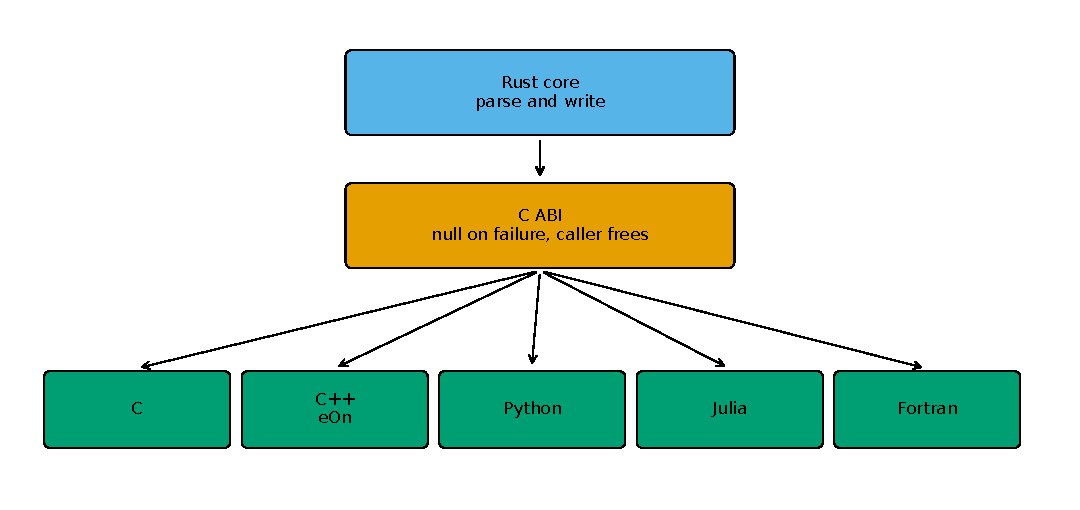
\includegraphics[width=0.92\textwidth]{figures/generated/architecture.pdf}
\caption{Layering of the reference implementation.
The Rust core parses and writes CON.
The C ABI is the waist every other caller uses, including the C++ wrapper that eOn 3.6.0 calls.
The diagram is the structure of this release.}
\label{fig:architecture}
\end{figure}

The caller owns a frame handle it received and frees the handle when it is finished, which is why Listing~\ref{lst:c} ends in a free of the whole array.
Structure-of-arrays accessors return a pointer into that frame, so the coordinates are not copied on the way out, and the pointer is not valid after the free.
Absent numeric metadata is a NaN sentinel: the energy accessor returns NaN when the frame has no energy, and that sentinel is not written back to a file.
ABI version macros (\texttt{RKR\_ABI\_VERSION\_MAJOR}, \texttt{RKR\_ABI\_VERSION\_MINOR}, \texttt{RKR\_ABI\_LAYOUT\_REVISION}) let a caller refuse a header whose layout it does not know.
The Rust core and the bindings built on it distinguish the error classes of Section~\ref{sec:format}.
The C bulk read does not.
It returns a null handle, as Listing~\ref{lst:c} tests, and the class that rejected the file is not available on that path.
Other C calls return status codes for a null pointer, a short buffer, an absent section and a disabled feature, and those codes are not a substitute for the parse class.
% CHECK: update if per-class C error codes ship on the read path.

\begin{lstlisting}[language=C,caption={Reading every frame through the C ABI. A failed read is a null handle. The energy accessor is NaN when the frame stores no energy. The caller frees the array.},label={lst:c}]
uintptr_t n = 0;
struct RKRConFrame **f = rkr_read_all_frames(path, &n);
if (f == NULL) { /* failure: null handle */ return 1; }
uintptr_t natoms = rkr_frame_atom_count(f[0]);
uintptr_t nxyz = 0;
const double *xyz = rkr_frame_xyz_f64(f[0], &nxyz);
double e = rkr_frame_energy(f[0]);   /* NaN when absent */
free_rkr_frame_array(f, n);          /* frees every frame */
\end{lstlisting}

Listing~\ref{lst:py} is the same contract from Python.
The default write is the round-trip printer, and six decimals are a separate argument.
An atom object exposes the symbol, the id, the per-axis mask and any velocity components, which is the surface a hand-off into ASE uses when the caller builds the ASE constraints from the mask rather than from a single freeze flag.
Fortran 2008 reaches the same C symbols through its C interoperability, and Julia does so through its foreign-function interface \cite{bezansonJuliaFreshApproach2017}.
The Python binding can also hand coordinates back as arrays, so a caller who does not want one object per atom is not forced to build them on every call \cite{harrisArrayProgrammingNumpy2020}.
The timed path in Section~\ref{sec:performance} is the object path.
We keep the split on purpose: a campaign that needs only coordinates should not pay for one object per atom, while a caller who wants the mask and the id on a named atom uses the object Listing~\ref{lst:py} constructs.
On a version 3 frame the builder stamps minor 1 when the caller set no minor, and it refuses velocities at that minor unless a time unit was supplied.
Unknown keys already stored on the frame are written back, which is how a bead index survives a round trip.

\begin{lstlisting}[language=Python,caption={Round-trip and opt-in six-decimal writes. The default printer is the one that preserves binary64.},label={lst:py}]
frames = readcon.read_con("slab.con")
a = frames[0].atoms[-1]          # symbol, atom_id, fixed (x,y,z), vx, vy, vz
readcon.write_con("rt.con", frames)               # round-trip printer
readcon.write_con("f6.con", frames, precision=6)  # lossy, opt-in
\end{lstlisting}

A multi-frame read finds frame boundaries before it builds atoms.
We scan the header counts in one pass and record the byte offset where each frame starts, the same idea as an on-disk offset index for a trajectory, and the scan stays serial because each start depends on the counts of every frame before it \cite{gowersMdanalysisPythonPackage2016}.
Workers therefore never race to find the next newline.
Once the offsets exist, each task parses only its own slice, the result array is filled at the index the scan assigned, and the hash of the frame contents is the same at every worker count.
Adding workers cannot reorder atoms or drop a frame, since the split does not depend on how many workers are waiting.
When the parallel feature is on, a file of at least 48\,KiB uses the pool, a smaller file stays on the serial path the one-thread timings measure, and a file that holds a single frame stays one task however many atoms it contains.
We ship the wheels and the C archives with that feature turned on.
Handles are per thread: a frame handle is used from the thread that received it, and it is not a shared mutable object.
The Python call releases the interpreter lock while the core parses, and it takes the lock back to construct the per-atom objects the listing shows.
The C archive and the Python wheel both contain that core, so the corpus a binding runs is a check of the same parse.

The same corpus of legal and illegal frames is what each binding runs, so a binding cannot quietly accept a file the core rejects.
Builds that want an ingress from other chemical files can link chemfiles, and that ingress is optional \cite{frauxChemfilesVersion01042023,frauxChemfiles2023}.
Symmetry libraries, descriptor libraries and collective-variable engines consume a geometry after the search, and they are not a second checkpoint \cite{togoSpglibSoftwareLibrary2024,himanenDscribeLibraryDescriptors2020,tribelloPlumed2New2014}.
Remote procedure calls, metatensor exchange and DLPack views are optional build features and are outside the claims of this paper \cite{bigiMetatensorMetatomicFoundational2026}.
The C ABI is the link a C-speaking electronic-structure code would use if it wanted the frame directly \cite{oliveiraCecamElectronicStructure2020}.
The C++ archive for this release, \texttt{readcon-core-cxx-0.17.0.tar.gz}, has SHA-256 \texttt{4bf6b1809da292a7ea5cc59376e57220f31afa052c7365aecdc3b039c70b52f3}.
Callers install that archive rather than a private build of the core.
An ASE atoms object can be copied into a frame.
In this release that copy takes an id array when the caller has set one and otherwise numbers atoms in row order, and it does not write the velocity time unit into the metadata of a version 3 frame, so a caller who has velocities must set the unit.
% CHECK: update if ASE ingress sets atom ids and the velocity time unit without a caller-supplied array.

\section{Validation}
\label{sec:validation}
We treat a frame as conformant when every binding agrees on whether it is legal, and we treat a restart as faithful when the geometry a search reloads matches the geometry that was stored.
The precedent for the first test is a shared validation list such as checkCIF, which turns a format rule into an alert a later reader can reproduce \cite{spekCheckcifValidationAlerts2020,hallCrystallographicInformationFile1991}.
Table~\ref{tab:corpus} is the corpus by category.
% TODO: corpus category counts
Legal frames, covering the header, both mask meanings, an empty frame and the units line, must be accepted.
Illegal frames, covering an unknown major, broken version-3 units, an illegal flag, an unknown section, strict validation without a section list, or a zero per-type count, must be rejected.
Agreement means that accept-or-reject decision.
It does not mean that every binding reports the same error class, which the C read path of Section~\ref{sec:implementation} cannot do.
% CHECK: update if identical error classes across bindings become part of the corpus.

\begin{table}[ht]
\centering
\small
\caption{Conformance corpus by category. Each binding runs the same files.}
\label{tab:corpus}
\begin{tabular}{p{0.24\linewidth}p{0.68\linewidth}}
\toprule
Category & What the binding must do \\
\midrule
Legal & Accept the frame, including both mask meanings, an empty frame and the units line. \\
Illegal & Reject the frame. \\
Cross-binding & Run the same files the Rust core runs. \\
\bottomrule
\end{tabular}
\end{table}

Bit-level round trips are the numeric half of that contract.
The eOn checkpoint written by the default printer in the restart below reads back bit-identical, and the six-decimal writer differs by a maximum of \(5.0\times10^{-7}\,\text{\AA}\).
The 218-atom frames of the timing set in Section~\ref{sec:performance} likewise match after a default rewrite, and the ASE reading of that producer file agrees on the coordinates.
The cross-reader check also includes the public HCN and HNC endpoints of the hydrogen cyanide isomerisation \cite{mourikAbInitioGlobal2001,goswamiReproducibleOrchestrationBest2026}.

Mask and identity are where the ASE reader and this library part company.
On the 28-atom Pt(100) slab, bottom layer mask 7 plus an adatom at mask 4, ASE 3.29.0 reports \texttt{FixAtoms} on indices 0 through 8 and 27, which freezes the adatom on every axis.
The adatom then cannot move laterally, so a band built from that reading cannot represent the hollow-to-hollow hop, and the frozen components change which modes enter the prefactor.
A quantitative ASE band on the two readings would require endpoints relaxed under each constraint set and an optimiser run to convergence, and that rerun is not what is reported here.
% CHECK: the ASE mask comparison stays qualitative until a converged rerun with endpoints relaxed under each constraint set.
Column 5 is kept by this library, so a caller pairs atoms by id after the file has grouped them by element, instead of by row.
The bindings return that id on the file-order atom, which is the surface Listing~\ref{lst:py} shows.

\subsection{An interrupted eOn band}
We restart an eOn 3.6.0 client with the Morse Pt potential and ASE 3.29.0, on a Pt(100) \(3\times3\times3\) slab plus one adatom (28 atoms, the bottom 9 at mask 7) \cite{goswamiEonV3602026,goswamiEnhancedClimbingImage2026}.
The event is a hollow-to-hollow hop, the band has five movable images, the optimiser is steepest descent, and both the uninterrupted run and each resume take five steepest-descent steps.\footnote{Giving the resume the same iteration cap as the uninterrupted job leaves it one step short, because iteration 0 writes the loaded band and does not step.
The \(0.0068\,\mathrm{eV}\) gap of that unmatched pair is the step count.}
Minimisations, the band and the dimer reported below all stop at an iteration cap.
The matched comparison is the primary result, and it is the band after those five steps.

We find that both resumed runs reproduce the uninterrupted printed table: max force \(3.0658\), then \(1.2007\), then \(0.59762\,\mathrm{eV}/\text{\AA}\), and highest image \(0.8305\), then \(0.6911\), then \(0.6417\,\mathrm{eV}\).
After the five steps the round-trip resume barrier is \(0.63493\,\mathrm{eV}\), a difference of 0 from the uninterrupted band.
On that final band the minimum-image displacement is at most \(8.9\times10^{-15}\,\text{\AA}\) (RMSD \(1.1\times10^{-15}\,\text{\AA}\)), which is agreement to \(1\times10^{-14}\,\text{\AA}\).
The six-decimal resume shifts the same barrier by \(+1.0\times10^{-6}\,\mathrm{eV}\), with a minimum-image maximum of \(4.9\times10^{-7}\,\text{\AA}\) and an RMSD of \(2.0\times10^{-7}\,\text{\AA}\).
The checkpoint round trip is the part that is bitwise exact.
The resumed band is not bitwise exact, because the search has taken steps after the load.
Figure~\ref{fig:restart} plots the shared printed series and the final-band displacements.
No point on that figure is missing.

\begin{figure}[ht]
\centering
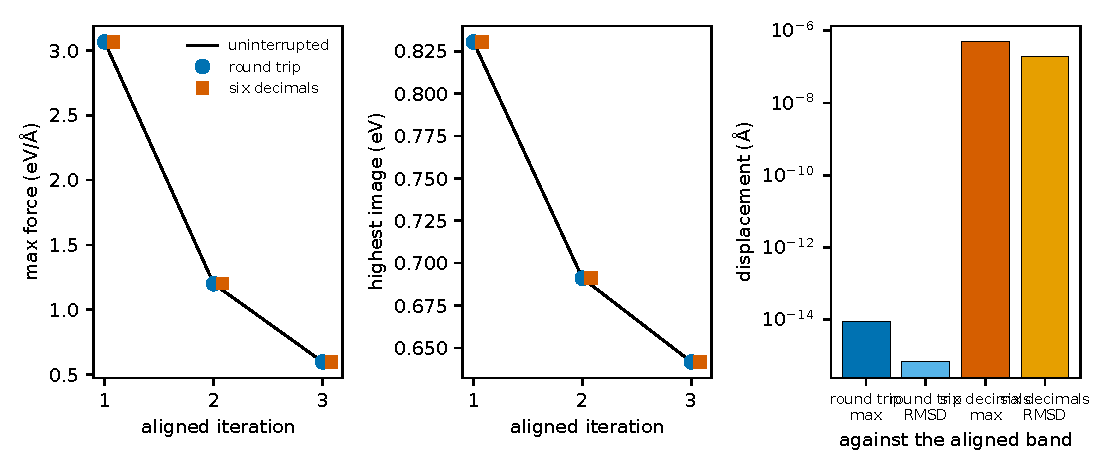
\includegraphics[width=\textwidth]{figures/generated/restart.pdf}
\caption{Interrupted eOn nudged elastic band on a 28-atom Pt(100) slab with a Morse potential, five movable images and steepest descent \cite{goswamiEonV3602026,goswamiEnhancedClimbingImage2026}.
Both the uninterrupted run and each resume take five steepest-descent steps, and the search stops at an iteration cap.}
Left and centre: max force and highest-image energy for the uninterrupted run and for resumes from a round-trip checkpoint and from a six-decimal checkpoint.
The three series coincide at printed precision.
Right: minimum-image maximum and RMSD of each final band against the uninterrupted band, on a logarithmic axis.
The round-trip barrier at that band is \(0.63493\,\mathrm{eV}\), with difference 0.}
\label{fig:restart}
\end{figure}

An L-BFGS control, which is eOn's default band optimiser, does not show the same split \cite{goswamiEonV3602026,goswamiEnhancedClimbingImage2026}.
Both checkpoints resume to \(0.6707\,\mathrm{eV}\) against \(0.6336\,\mathrm{eV}\) for the uninterrupted ending, since the limited-memory history is not in a geometry checkpoint and the two files therefore lose the same thing.
A dimer started from the round-trip geometry gives a saddle energy of \(-112.618941\,\mathrm{eV}\) and a curvature of \(-10.613681\), identical to the plain run \cite{goswamiEonV3602026,goswamiEfficientExplorationChemical2025}.
Six decimals shift that saddle by \(-3.0\times10^{-6}\,\mathrm{eV}\), to a curvature of \(-10.613677\), with a positional RMSD of \(5.4\times10^{-7}\,\text{\AA}\).
The dimer, like the band, stops at its iteration cap.

The velocity numbers are a separate illustration, not a second restart.
On the same 28 atoms at 300\,K the kinetic energy is \(0.888\,\mathrm{eV}\) in the natural unit and \(92.02\,\mathrm{eV}\) if those components are misread as \(\text{\AA}/\mathrm{fs}\), a ratio of \(103.64=(10.1805)^{2}\).
One velocity Verlet step of \(1\,\mathrm{fs}\) with the ASE EMT potential then misplaces atoms by an RMSD of \(0.096\,\text{\AA}\) (maximum \(0.315\,\text{\AA}\)).
The velocity round trip itself is exact.
eOn's dynamics job redraws velocities and writes none, so there is no eOn velocity restart to compare, and the factor is evidence of what the 3.0 label did to a reader rather than evidence that a dynamics checkpoint was reloaded.

\section{Performance}
\label{sec:performance}
We time three layers on one file, on an Intel Xeon processor of family 6, model 207, with 8 hardware threads, compiled with rustc 1.88 and g++ 13.3 and run under Python 3.12.
The file is \(167.71\,\mathrm{MB}\), 10{,}000 frames of 218 atoms, and the cache is warm.
We report the median together with a bias-corrected and accelerated 95 percent interval \cite{efronBetterBootstrapConfidence1987,kaliberaRigorousBenchmarkingReasonable2013,mytkowiczProducingWrongData2009,hoeflerScientificBenchmarkingParallel2015}.
Table~\ref{tab:perf} and Figure~\ref{fig:layers} are those medians.
The C++ column is the wrapper eOn calls, so the ratio against Rust is wrapper overhead rather than a contest with a second parser.

\begin{table}[ht]
\centering
\small
\caption{Layered timings on the 10{,}000-frame file.
Frames per second for rows other than the Rust core are 10{,}000 divided by the median time, rounded.
The Rust interval is the bias-corrected 95 percent interval of the median.}
\label{tab:perf}
\begin{tabular}{lrrrr}
\toprule
Layer & Threads & Time (s) & MB/s & frames/s \\
\midrule
Rust core & automatic & 0.154 [0.149, 0.160] & 1{,}090 & 64{,}970 \\
C++ wrapper & automatic & 0.156 & 1{,}078 & 64{,}100 \\
Rust core & 1 & 0.551 & 304 & 18{,}100 \\
C++ wrapper & 1 & 0.527 & & 19{,}000 \\
Python objects & & 1.369 & 122.5 & 7{,}300 \\
ASE reader & & 3.856 & 43.5 & 2{,}600 \\
\bottomrule
\end{tabular}
\end{table}

\begin{figure}[ht]
\centering
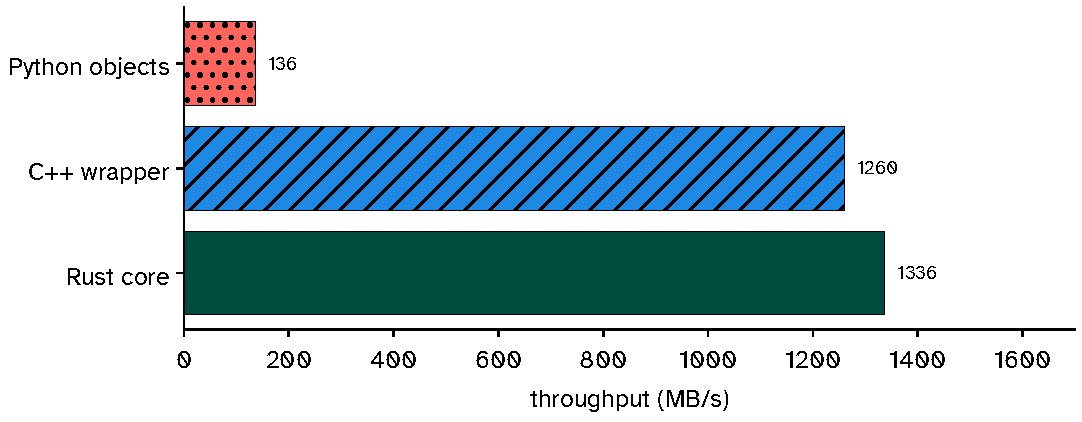
\includegraphics[width=0.78\textwidth]{figures/generated/layers.pdf}
\caption{Median throughput on a \(167.71\,\mathrm{MB}\) file of 10{,}000 frames of 218 atoms, warm cache.
The Rust core and the C++ wrapper, which is the reader eOn calls, sit near \(1.09\,\mathrm{GB/s}\).
The Python bar includes construction of one object per atom.}
\label{fig:layers}
\end{figure}

At the automatic width the Rust time is \(0.988\) of the C++ time, interval \([0.942, 0.989]\).
On one thread that ratio is \(1.016\), interval \([0.965, 1.142]\), so the wrapper is not a large fraction of the parse in either direction.
The \(0.100\,\mathrm{s}\) stage loads the bytes into a string, a copy plus a UTF-8 check, and it is not an I/O floor.
Copying the file to the null device on a hot page cache takes \(0.0212\,\mathrm{s}\) (\(7.9\,\mathrm{GB/s}\)).
The eight-thread parse is about \(7.7\) times that floor.
The serial string load and the boundary scan, \(0.100\,\mathrm{s}\) and \(0.036\,\mathrm{s}\), limit scaling, which is what Amdahl's law gives for a speedup of \(3.8\) on 8 threads.
% CHECK: confirm the serial fraction behind ``3.8 on 8 threads'' before that Amdahl clause is left as a result.
Python full objects take \(1.369\,\mathrm{s}\) (\(122.5\,\mathrm{MB/s}\)) against \(3.856\,\mathrm{s}\) (\(43.5\,\mathrm{MB/s}\)) for the ASE reader of the same text, a ratio of \(0.351\) with interval \([0.335, 0.379]\), about \(2.8\) times, and the positions-only ratio is \(0.342\) with interval \([0.335, 0.357]\).
Object construction is about \(0.826\,\mathrm{s}\), interval \([0.725, 0.851]\), roughly 60 percent of the Python time.
That estimate subtracts the one-thread Rust parse from the Python read at the same repeat index, and the two blocks were sequential, so the difference is index-aligned rather than an interleaved pair.

Speedup at 1, 2, 4 and 8 threads is 1.00, 1.61, 2.73, 3.78 for Rust, 1.00, 1.39, 2.36, 3.26 for C++, and 1.00, 1.15, 1.22, 1.08 for Python.
The Python curve flattens because object construction holds the interpreter lock, not because the boundary scan has run out of work, and the measurement stops at 8 threads because that is the hardware.
Figure~\ref{fig:scaling} in Appendix~\ref{sec:appendix-bench} draws the three curves.
A force-call framing, in the style of the i-PI 3.0 measurements, puts the same file next to the evaluator it is waiting on \cite{litmanIpi30Flexible2024}.
One 218-atom frame reads in \(15\,\mu\mathrm{s}\).
One Morse call on the 28-atom slab takes \(0.30\,\mathrm{ms}\), one EMT call takes \(59\,\mu\mathrm{s}\), and a DFT call takes seconds to minutes.
The whole file costs about 510 Morse calls.
On an earlier round of the same 10{,}000-frame band, with different fields in the peer files, chemfiles reading XYZ was \(2.15\) times faster, h5py reading one position array was \(67\) times faster, and MDAnalysis reading H5MD was \(4.8\) times slower \cite{michaudagrawalMdanalysisToolkitAnalysis2011,jakupovicMpiparallelMolecularDynamics2021,gowersMdanalysisRelease21002025}.
% CITE-NEEDED: h5py has no DOI in the citation list.

\section{Limitations and outlook}
\label{sec:limitations}
A geometry checkpoint does not contain optimiser history, so an L-BFGS resume matches the atoms and not the quasi-Newton memory, as the control in Section~\ref{sec:validation} shows for both printers alike.
Python pays for per-atom objects under the interpreter lock, which is most of the Python time in Table~\ref{tab:perf}, and a caller who needs only coordinates can stay on the array accessors instead.
The C bulk read returns a null handle with no error class, so a C caller learns that the file failed and not which rule it broke.
The scaling measurement uses 8 hardware threads on one processor, and no claim is made for a larger machine.
The Python binding is not a free-threaded build, so the plateau in Figure~\ref{fig:scaling} is an interpreter limit rather than a property of the scan, and a rebuild against a free-threaded interpreter would be a later measurement.
We expect the next minor to add a section under the rules of Section~\ref{sec:format}, without a new major and without a flag day for files already written.
An H5MD export would serve a band that has outgrown text, once slicing matters more than a diff, and that bridge is not part of this release.
Adoption in ASE would retire the mask collapse in the reader that currently freezes a nonzero column, and that change belongs in ASE rather than in a second reading hidden here.
Both directions are open to contribution, provided a change stays inside the compatibility promise that keeps 3.1 stable after the seven months in which the four versions were written down.
A store of frames for adaptive kinetic Monte Carlo queries is a separate project, sketched in Appendix~\ref{sec:appendix-db}, and it does not alter the frame.
Publishing a finished saddle remains the job of a repository interface and a materials archive, downstream of the checkpoint rather than a replacement for it \cite{andersenOptimadeApiExchanging2021,draxlNomadLaboratoryData2019}.

\section{Conclusions}
\label{sec:conclusions}
CON 3.1 specifies the text checkpoint that eOn and ASE exchange, including the per-axis mask, the atom identity and the velocity time unit that readers have been dropping.
readcon-core 0.17.0 is the reference implementation, and eOn 3.6.0 reads CON through it.
An interrupted band resumed from the default printer agrees with the uninterrupted band to \(1\times10^{-14}\,\text{\AA}\), against a drift of \(5\times10^{-7}\,\text{\AA}\) at six decimals, and the core reads at 1.09\,GB/s beside a force call that dominates the campaign.
The conformance corpus is what each binding runs against that specification.

\section*{Data availability}
\label{sec:data}
The version 0.17.0 archive is \url{https://doi.org/10.5281/zenodo.23302640} \cite{goswamiReadconcoreV0170Conconvel2026}, and the concept record that collects every version is \url{https://doi.org/10.5281/zenodo.18753567} \cite{goswamiReadconcoreConConvel2026}.
A citation to research software is owed to the archived record, and the archive is the object the software principles ask an author to identify \cite{smithSoftwareCitationPrinciples2016,wilkinsonFairGuidingPrinciples2016,barkerIntroducingFairPrinciples2022,lamprechtFairPrinciplesResearch2020}.
The HCN and HNC endpoints used in the cross-reader check are the public files of that workflow study \cite{goswamiReproducibleOrchestrationBest2026}.
The normative specification, the grammar, the schema, the conformance corpus and the evidence scripts are the supplementary material.

\section*{CRediT authorship contribution statement}
\label{sec:credit}
Rohit Goswami: Conceptualization, Methodology, Software, Visualization, Writing - Original draft preparation, Writing - Reviewing and Editing.

\section*{Declaration of competing interest}
\label{sec:competing}
The author declares that he has no known competing financial interests or personal relationships that could have appeared to influence the work reported in this paper.

\section*{Funding}
\label{sec:funding}
This work received no funding.

\section*{Acknowledgements}
\label{sec:acknowledgements}
The author thanks Hannes J{\'o}nsson for long discussions on saddle searches and on what an eOn checkpoint has to carry, and Miha Gunde for discussions on matching atoms along a reaction path.
Ruhila Goswami designed the colour palette of the figures.
The library was written with the patience of the author's family, in the company of the turtles, the garden cats, the birds and the rest of the household.

\appendix

\section{Benchmark protocol}
\label{sec:appendix-bench}
The processor, the compiler versions and the warm-cache condition are those of Section~\ref{sec:performance}.
Each reported time is a median, and the interval is a bias-corrected and accelerated bootstrap at 95 percent \cite{efronBetterBootstrapConfidence1987}.
Repeats are the unit the interval is built from, which is the practice that keeps a benchmark from reporting a single lucky run as a rate \cite{kaliberaRigorousBenchmarkingReasonable2013,mytkowiczProducingWrongData2009,hoeflerScientificBenchmarkingParallel2015}.
The Python object estimate is index-aligned across two sequential blocks, and it is not an interleaved pair, so it is labelled as an estimate in the main text.
Figure~\ref{fig:scaling} is the speedup at 1, 2, 4 and 8 threads.\footnote{A step-down correction across many ratios \cite{holmStepdown1979} is not applied.
The intervals in Section~\ref{sec:performance} are for a few predeclared layers, not a search over peers.}

\begin{figure}[ht]
\centering
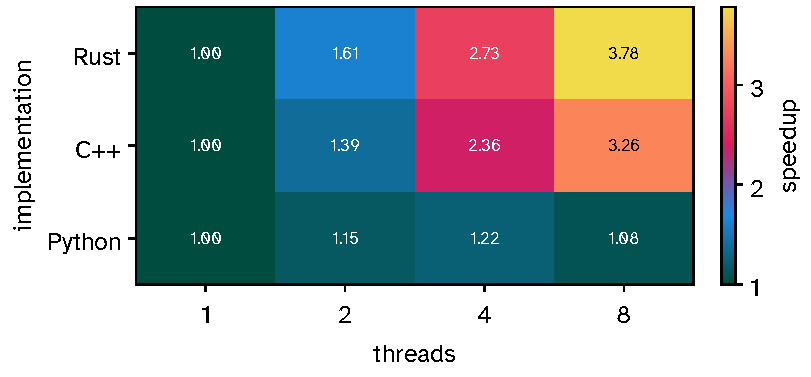
\includegraphics[width=0.62\textwidth]{figures/generated/scaling.pdf}
\caption{Speedup against a one-thread baseline on the 10{,}000-frame file, for the Rust core, the C++ wrapper and the Python object path.
The dashed line is ideal scaling.
Python flattens because object construction holds the interpreter lock.
The measurement stops at 8 threads.}
\label{fig:scaling}
\end{figure}

\section{Reader edge-case rules}
\label{sec:appendix-rules}
Table~\ref{tab:rules} collects the edge cases a reader applies.
They are the same classes as Section~\ref{sec:format}, stated as input and outcome so that a binding can be checked against them.

\begin{table}[ht]
\centering
\small
\caption{Reader rules for flags, versions, identity and incomplete input.}
\label{tab:rules}
\begin{tabular}{p{0.46\linewidth}p{0.48\linewidth}}
\toprule
Input & Rule \\
\midrule
Column 4 outside the legal set, any mode & Illegal flag. \\
Version 1 column 4 equal to 1 & Fixed on \(x\), \(y\) and \(z\). \\
Version 1 column 4 other than 0 or 1 & Illegal flag. \\
Missing id column & Id is the zero-based row index. \\
Repeated id & File order is kept. \\
Unique ids & Ascending id is the pre-grouping order. \\
Unknown major & Rejected. \\
Unknown minor of a known major & Accepted. \\
Unknown metadata key & Kept on rewrite. \\
Unknown section at this minor & Rejected. \\
Unknown section at a newer minor, width declared & May be skipped. \\
Non-finite number, any mode & Rejected. \\
Type count of zero & Legal empty frame. \\
Short header or short section & No partial frame is returned. \\
Several gzip members & Read in order. \\
\bottomrule
\end{tabular}
\end{table}

\section{readcon-db}
\label{sec:appendix-db}
A store of CON frames and saddles would let an adaptive kinetic Monte Carlo campaign query the checkpoints it has already written, rather than scanning a directory of text after the fact.
Reaction databases, catalysis archives, Open Catalyst records kept on LMDB, a barrier dataset and a materials API are the precedents for that kind of collection \cite{terrellDatabaseAtomisticReaction2012,wintherCatalysishuborgOpenElectronic2019,chanussotOpenCatalyst20202021,schreinerTransition1xDatasetBuilding2022,ongMaterialsApplicationProgramming2015}.
A chunked array specification is a different object from an index of frames \cite{opengeospatialconsortiumZarrStorageSpecification2022}.
% TODO readcon-db results

\section{ABNF of one frame}
\label{sec:appendix-abnf}
The non-normative grammar of one frame is inserted here.
\begin{lstlisting}[caption={Non-normative ABNF for one frame.},label={lst:abnf}]
file = [bom] 1*frame *(*ws nl)
bom = %xFEFF
header_open = free_line nl metadata_line nl float3_line float3_line free_line nl free_line nl
frame = header_open (zero_atom / typed_body)
free_line = *(%x00-09 / %x0B-0C / %x0E-FF)
metadata_line = *ws (json_object / legacy_metadata)
legacy_metadata = *ws free_line
json_object = "{" *ws [json_pair *(*ws "," *ws json_pair)] *ws "}" *ws
json_pair = json_string *ws ":" *ws json_value
json_value = json_string / json_number / json_object / json_array / "true" / "false" / "null"
json_array = "[" *ws [json_value *(*ws "," *ws json_value)] *ws "]"
json_string = DQUOTE *json_char DQUOTE
json_char = "\" DQUOTE / "\\" / "\/" / "\b" / "\f" / "\n" / "\r" / "\t" / ("\u" 4HEXDIG) / (%x20-21 / %x23-5B / %x5D-FF)
json_number = ["-"] 1*DIGIT ["." 1*DIGIT] [("e" / "E") ["+" / "-"] 1*DIGIT]
float3_line = *ws float 1*ws float 1*ws float *ws nl
count_line = *ws positive_integer *ws nl
count_list_line = *ws positive_integer *(1*ws positive_integer) *ws nl
float_list_line = *ws float *(1*ws float) *ws nl
zero_integer = 1*"0"
zero_count_line = *ws zero_integer *ws [nl]
blank_line = *ws nl
zero_atom = zero_count_line (blank_line (blank_line / "") / "")
typed_body = count_line count_list_line float_list_line 1*type_block *section
type_block = symbol_line nl coord_label nl vector_atom_line *(nl vector_atom_line) [nl]
symbol_line = *ws symbol *ws
symbol = ALPHA *(ALPHA / DIGIT / "_")
coord_label = *ws "Coordinates of Component" 1*ws positive_integer *ws
vector_atom_line = *ws float 1*ws float 1*ws float 1*ws integer [1*ws integer] *ws
scalar_atom_line = *ws float 1*ws integer 1*ws integer *ws
atom_line = vector_atom_line
section = *ws nl (1*section_type_block_vector / 1*section_type_block_scalar / 1*generic_type_block)
section_type_block_vector = symbol_line nl section_label_vector nl vector_section_line *(nl vector_section_line) [nl]
section_type_block_scalar = symbol_line nl section_label_scalar nl scalar_atom_line *(nl scalar_atom_line) [nl]
generic_type_block = symbol_line nl generic_label nl token_line *(nl token_line) [nl]
generic_label = *ws symbol *(1*ws (symbol / positive_integer)) *ws
token_line = *ws (float / integer) *(1*ws (float / integer)) *ws
vector_section_line = *ws float 1*ws float 1*ws float 1*ws integer 1*ws integer *ws
section_kind_vector = "Velocities" / "Forces" / "Magmoms" / "Displacements" / "Spreads"
section_kind_scalar = "Energies" / "Charges" / "Spins"
section_kind = section_kind_vector / section_kind_scalar
section_label_vector = *ws section_kind_vector 1*ws "of Component" 1*ws positive_integer *ws
section_label_scalar = *ws section_kind_scalar 1*ws "of Component" 1*ws positive_integer *ws
float = finite_float / non_finite
finite_float = ["+" / "-"] (1*DIGIT ["." *DIGIT] / "." 1*DIGIT) [("e" / "E") ["+" / "-"] 1*DIGIT]
non_finite = ["+" / "-"] ("infinity" / "nan" / "inf")
integer = 1*DIGIT
positive_integer = (%x31-39) *DIGIT
ws = SP / HTAB
NL = CRLF / LF
nl = NL
\end{lstlisting}


\bibliographystyle{elsarticle-num}
\begingroup\catcode`\&=12
\bibliography{rg_main}
\endgroup
\end{document}
